%=================== LaTeX 习题模板(仅含学院与考试信息) ===================
\documentclass[12pt,a4paper]{article}

%----------------- 页面与中文支持 -----------------
\usepackage[margin=2cm]{geometry}    % 设置页边距
\usepackage{ctex}                    % 支持中文
\usepackage{amsmath,amssymb}         % 数学公式与符号
\usepackage{enumitem}                % 自定义列表格式
\usepackage{tikz}
\usetikzlibrary{decorations.pathmorphing}
\usepackage{float} % 支持 [H] 浮动体选项

%----------------- 页眉页脚 -----------------
\usepackage{fancyhdr}
\pagestyle{fancy}
\fancyhf{}
% 左侧:学院(留空由学生填写)
\lhead{学院:\underline{\hspace{2cm}建工学院\hspace{2cm}}}
% 右侧:考试信息(如“期末考试”、“月考试卷”等,由学生填写)
\rhead{考试:\underline{\hspace{2cm}材料力学\hspace{2cm}}}
\cfoot{\thepage}

%----------------- 题目环境 -----------------
\newcounter{question}
\newenvironment{questions}{
    \setcounter{question}{0}
    \section*{习题(题目)}
    \begin{enumerate}[leftmargin=1.5em,label={\arabic*.}]
}{
    \end{enumerate}
}

%----------------- 答案环境 -----------------
\newenvironment{answers}{
    \setcounter{question}{0}
    \section*{习题答案}
    \begin{enumerate}[leftmargin=1.5em,label={\arabic*.}]
}{
    \end{enumerate}
}

% 用于每题答案的加粗提示
\newcommand{\answer}[1]{\par\noindent\textbf{答案:} #1\par\vspace{1em}}

%=========================================================

\begin{document}

\section*{1. 轴向拉伸/压缩}

\begin{align}
& N \quad\text{—— 轴向内力(拉力为正,压缩为负)},\\
& \sigma \;=\; \frac{F}{A},\\
& \varepsilon \;=\; \frac{\sigma}{E} \;=\; \frac{F}{A\,E},\\
& \delta \;=\; \varepsilon\,L \;=\; \frac{F\,L}{A\,E},\\
& u \;=\; \int_{0}^{\varepsilon} \sigma\,d\varepsilon \;=\; \frac{1}{2}E\,\varepsilon^2 
      \;=\; \frac{\sigma^2}{2\,E} 
      \;=\; \frac{F^2}{2\,A\,E},\\
& U \;=\; u\,(A\,L) \;=\; \frac{F^2\,L}{2\,A\,E}.
\end{align}

\section*{2. 固定端扭转(圆轴扭转)}

\begin{align}
& T \quad\text{—— 扭矩(顺时针为正)},\\
& \tau(\rho) \;=\; \frac{T\,\rho}{I}, 
    \quad \tau_{\max} \;=\; \frac{T\,r}{I},\\
& \theta \;=\; \frac{T\,L}{G\,I},\\
& \gamma(\rho) \;=\; \frac{\rho}{L}\,\theta \;=\; \frac{T\,\rho}{G\,I},\\
& U \;=\; \int_{0}^{L} \Bigl(\int_{A} \frac{\tau^2}{2\,G}\,dA \Bigr)\,dx 
      \;=\; \frac{T^2\,L}{2\,G\,I_\rho}.
\end{align}

\section*{3. 纯弯曲(直梁截面弯曲)}

\begin{align}
& M \quad\text{—— 弯矩(正方向按右手定则)},\\
& \sigma_b(y) \;=\; \frac{M\,y}{I_z}, 
    \quad \text{其中 }I_y\text{ 为绕中性轴的截面惯性矩},\\
& \kappa \;=\; \frac{1}{\rho} \;=\; \frac{M}{E\,I_z}, 
    \quad \rho \;=\; \frac{E\,I_z}{M},\\
& \frac{d^2 w}{d x^2} \;=\; \frac{M(x)}{E\,I_z},\\
& u \;=\; \int_{0}^{\varepsilon_b} \sigma_b\,d\varepsilon_b 
      \;=\; \int_{0}^{\sigma_b} \frac{\sigma}{E}\,d\sigma 
      \;=\; \frac{\sigma_b^2}{2\,E} 
      \;=\; \frac{M^2\,y^2}{2\,E\,I_z^{2}},\\
& U \;=\; \int_{0}^{L} \Bigl(\int_{A} \frac{\sigma_b^2}{2\,E}\,dA \Bigr)\,dx 
      \;=\; \int_{0}^{L} \frac{M(x)^2}{2\,E\,I_z}\,dx.
\end{align}

\section*{4. 组合工况总应变能}

若杆件同时受轴向力 \(N\)、弯矩 \(M(x)\)、扭矩 \(T\),且截面各参数视为常数,则应变能叠加:
\[
U_{\text{总}} \;=\; 
\underbrace{\frac{N^2\,L}{2\,A\,E}}_{U_{\text{轴向}}}
\;+\; 
\underbrace{\int_{0}^{L} \frac{M(x)^2}{2\,E\,I_z}\,dx}_{U_{\text{弯曲}}}
\;+\; 
\underbrace{\frac{T^2\,L}{2\,G\,I}}_{U_{\text{扭转}}}.
\]
若截面沿长度变化,则保留积分形式:
\begin{align}
U_{\text{轴向}} &= \int_{0}^{L} \frac{N^2}{2\,A(x)\,E}\,dx,\\
U_{\text{弯曲}} &= \int_{0}^{L} \frac{M(x)^2}{2\,E\,I_z(x)}\,dx,\\
U_{\text{扭转}} &= \int_{0}^{L} \frac{T^2}{2\,G\,I(x)}\,dx.
\end{align}

\section*{5. 常用截面参数(附录)}

\subsection*{1. 矩形截面(宽 $b$,高 $h$)}
\begin{align}
  A &= b\,h, \\[6pt]
  I_y \;=\; \frac{b\,h^3}{12}, 
    &\quad &\text{(绕竖直 $y$ 轴的惯性矩)},\\[6pt]
  I_z \;=\; \frac{h\,b^3}{12}, 
    &\quad &\text{(绕水平 $z$ 轴的惯性矩)},\\[6pt]
  W_y \;=\; \frac{I_y}{h/2} 
    \;=\; \frac{b\,h^3}{12}\,\Big/\frac{h}{2} 
    \;=\; \frac{b\,h^2}{6}, 
    &\quad &\text{(绕 $y$ 轴的截面模数)},\\[6pt]
  W_z \;=\; \frac{I_z}{b/2} 
    \;=\; \frac{h\,b^3}{12}\,\Big/\frac{b}{2} 
    \;=\; \frac{h\,b^2}{6}, 
    &\quad &\text{(绕 $z$ 轴的截面模数)},\\[6pt]
  i_y \;=\; \sqrt{\frac{I_y}{A}} 
    \;=\; \sqrt{\frac{\tfrac{b\,h^3}{12}}{b\,h}} 
    \;=\; \frac{h}{\sqrt{12}}, 
    &\quad &\text{(绕 $y$ 轴的回转半径)},\\[6pt]
  i_z \;=\; \sqrt{\frac{I_z}{A}} 
    \;=\; \sqrt{\frac{\tfrac{h\,b^3}{12}}{b\,h}} 
    \;=\; \frac{b}{\sqrt{12}}, 
    &\quad &\text{(绕 $z$ 轴的回转半径)}.
\end{align}

\subsection*{2. 圆形截面(半径 $R$)}
\begin{align}
  A &= \pi\,R^2, \\[6pt]
  I_y = I_z \;=\; \frac{\pi\,R^4}{4} \; = \frac{\pi d^4}{32}, 
    &\quad &\text{(绕任意通过截面中心的直径方向)},\\[6pt]
  W_y = W_z \;=\; \frac{I_y}{R} 
    \;=\; \frac{\pi\,R^4}{4}\,\Big/R 
    \;=\; \frac{\pi\,R^3}{4}, 
    &\quad &\text{(截面模数)},\\[6pt]
  i_y = i_z \;=\; \sqrt{\frac{I_y}{A}} 
    \;=\; \sqrt{\frac{\tfrac{\pi\,R^4}{4}}{\pi\,R^2}} 
    \;=\; \frac{R}{2}.
\end{align}

这里给出三角形的惯性矩的推导:

\begin{figure}[H]
\centering
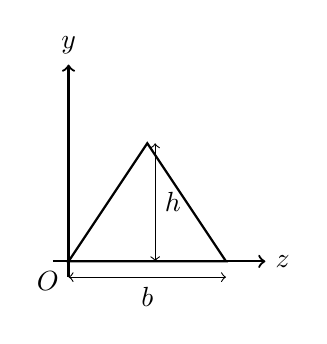
\begin{tikzpicture}
  
  % 坐标轴
  \draw[->, thick] (-0.2,0) -- (2.5,0) node[right] {$z$};
  \draw[->, thick] (0,-0.2) -- (0,2.5) node[above] {$y$};
  \node at (0,0) [below left] {$O$}; % 原点

  % 三角形顶点
  \def\a{2} % 底边长度
  \def\b{1.5} % 高度
  \draw[thick] (0,0) -- (\a,0) -- (\a/2,\b) -- cycle; % 三角形

  % 标注底边和高度
  \draw[<->] (0,-0.2) -- (\a, -0.2) node[midway, below] {$b$};
  \draw[<->] (\a/2 + 0.1, 0) -- (\a/2 + 0.1, \b) node[midway, right] {$h$};
\end{tikzpicture}
\end{figure}


首先我们知道了矩形的惯性矩公式:
$$
I_y = \frac{h\,b^3}{12}, \quad I_z = \frac{b\,h^3}{12}.
$$
对于三角形,两个三角形可以拼接为一个平行四边形,而平行四边形的惯性矩等于矩形。
但是我们计算的三角形形心的惯性矩,这里要使用下平行轴定理:
$$2(I_{z\text{三角形}}+\frac{1}{2}bh\times (\frac{1}{6}h)^2)=\frac{1}{12}bh^3$$
解得$I_{z\text{三角形}}=\frac{1}{36}bh^3$:
\subsection*{3. 工字钢截面(示意)}
工字钢截面形状较为复杂,一般分箱体域分段积分后求出:
\[
  I_y = \sum\limits_{\text{翼缘、腹板}} I_{y,\text{分段}}, 
  \quad
  I_z = \sum\limits_{\text{翼缘、腹板}} I_{z,\text{分段}},
\]
各分段按平行轴定理或差减法计算。截面模数:
\[
  W_y = \frac{I_y}{y_{\max}}, 
  \quad
  W_z = \frac{I_z}{z_{\max}},
\]
其中 $y_{\max}$ 为截面外缘距 $y$ 轴的最大距离,$z_{\max}$ 为距 $z$ 轴的最大距离。

\bigskip
\hrule
\bigskip

\section*{矩形截面与坐标轴示意图(TikZ)}

\begin{figure}[h]
\centering
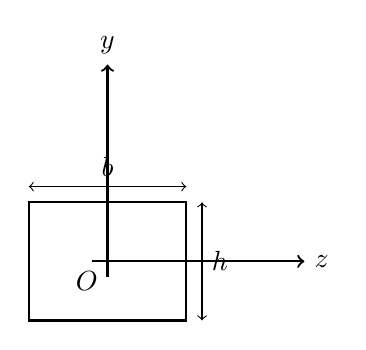
\begin{tikzpicture}[scale=1]
  % 坐标轴
  \draw[->, thick] (-0.2,0) -- (2.5,0) node[right] {$z$};
  \draw[->, thick] (0,-0.2) -- (0,2.5) node[above] {$y$};
  \node at (0,0) [below left] {$O$}; % 原点

  % 矩形截面(中心在原点,宽 b, 高 h)
  % 这里假设 b=2,h=1.5,用单位长度表示,实际编译时可按比例调整
  \def\b{2}
  \def\h{1.5}
  \draw[thick] (\b/2, \h/2) rectangle (-\b/2, -\h/2);

  % 标注尺寸 b (沿 z 轴)
  \draw[<->] (-\b/2, \h/2 + 0.2) -- (\b/2, \h/2 + 0.2) 
    node[midway, above] {$b$};

  % 标注尺寸 h (沿 y 轴)
  \draw[<->] (\b/2 + 0.2, -\h/2) -- (\b/2 + 0.2, \h/2) 
    node[midway, right] {$h$};
\end{tikzpicture}
\caption{矩形截面示意图:水平方向为 $z$ 轴,竖直方向为 $y$ 轴,中心为原点 $O$。}
\end{figure}

% 下面按前述格式,继续输出欧拉屈曲公式的内容,包括基本假设、临界载荷、临界应力、长细比、支撑条件下的 K 值以及示意图。

\section*{6. 欧拉屈曲公式}

\subsection*{6.1 临界屈曲载荷和应力}
\begin{align}
  P_{cr} 
  &= \frac{\pi^2\,E\,I}{(K\,L)^2}, 
  \quad\text{(欧拉临界屈曲载荷)}, \\[8pt]
  \sigma_{cr} 
  &= \frac{P_{cr}}{A} 
  = \frac{\pi^2\,E\,I}{A\,(K\,L)^2} 
  = \frac{\pi^2\,E}{\lambda^2}, 
  \quad \text{其中 } \lambda = \frac{K\,L}{r}, 
  \; i = \sqrt{\frac{I}{A}}.
\end{align}

\noindent 若 $\lambda \le \lambda_0$,则柱在屈曲前可能先发生屈服,需比较 $\sigma_{cr}$ 与材料屈服强度 $\sigma_y$。
\[
  \lambda_0 
  = \pi \sqrt{\frac{E}{\sigma_y}}, 
  \quad\text{(屈曲与屈服的分界长细比)}.
\]

\subsection*{6.2 支撑条件与等效长度系数 $K$}
在不同支撑条件下,柱的等效长度系数 $K$ 如下表所示:
\[
\begin{array}{|c|c|c|c|}
\hline
\text{支撑条件} & \text{两端铰支} & \text{一端固接,一端自由} & \text{两端固接} \\
\hline
K & 1.0 & 2.0 & 0.7 \\
\hline
\text{示意图} & 
\begin{minipage}{2.8cm}
\centering
\begin{tikzpicture}[scale=0.8]
  \draw[line width=1pt] (0,0) -- (0,2); 
  \draw[decorate,decoration={zigzag,segment length=3pt,amplitude=1pt}] (0,0) -- (0,-0.3); 
  \draw[decorate,decoration={zigzag,segment length=3pt,amplitude=1pt}] (0,2) -- (0,2.3); 
  \node at (0,-0.5) {铰支}; 
\end{tikzpicture}
\end{minipage}
&
\begin{minipage}{2.8cm}
\centering
\begin{tikzpicture}[scale=0.8]
  \draw[line width=1pt] (0,0) -- (0,2); 
  \draw[decorate,decoration={zigzag,segment length=3pt,amplitude=1pt}] (0,0) -- (0,-0.3); 
  \draw[fill,black] (0,2) circle (0.08); 
  \node at (0,-0.5) {一端固接\ \ \ 自由}; 
\end{tikzpicture}
\end{minipage}
&
\begin{minipage}{2.8cm}
\centering
\begin{tikzpicture}[scale=0.8]
  \draw[line width=1pt] (0,0) -- (0,2); 
  \draw[fill,black] (0,0) circle (0.08); 
  \draw[fill,black] (0,2) circle (0.08); 
  \node at (0,-0.5) {两端固接}; 
\end{tikzpicture}
\end{minipage}
\\
\hline
\end{array}
\]

\noindent 其中:
\begin{itemize}
  \item \textbf{两端铰支}:两端可自由转动,无弯矩约束,此时 $K = 1.0$。折曲形状为半个正弦。
  \item \textbf{一端固接,一端自由}:一端固接,另一端自由悬臂,此时 $K = 2.0$。折曲形状为完整肘形。
  \item \textbf{两端固接}:两端均固定(无转动),此时 $K \approx 0.7$。精确值为 $K = 0.699\ldots$,常取 $0.7$。
\end{itemize}

\subsection*{6.4 屈曲长细比与失稳准则}
\begin{itemize}
  \item 屈曲长细比:$\displaystyle \lambda = \frac{K\,L}{i} = \frac{K\,L}{\sqrt{I/A}}$。当 $\lambda$ 大于某临界值时,柱以屈曲方式失稳。
  \item 当 $\lambda \le \lambda_0 = \pi \sqrt{\dfrac{E}{\sigma_y}}$ 时,柱在压缩达到屈服前就会先屈服,此时不采用欧拉公式,而以材料屈服强度作为极限。
  \item 当 $\lambda > \lambda_0$ 时,柱会先发生弹性屈曲,临界载荷可用欧拉公式计算。
\end{itemize}

\section*{7.  纯弯曲挠度微分关系}

\subsection*{7.1 符号说明}
\begin{itemize}
  \item $x$:梁的坐标轴,沿梁长度方向。
  \item $w(x)$:梁在 $x$ 处的挠度(垂直位移),通常垂直于轴线,向下为正。
  \item $M(x)$:梁截面处的弯矩函数(关于中性轴)。
  \item $E$:材料杨氏模量。
  \item $I_z$:截面对中性轴的惯性矩。
\end{itemize}

\subsection*{7.2 挠度微分关系}
在纯弯曲条件下(梁仅受弯矩作用,无轴向力、剪力或扭矩干扰),根据平截面假设和线性弹性,梁的挠度满足如下二阶微分方程:
\[
  \frac{d^2 w(x)}{d x^2}
  \;=\;
  -\frac{M(x)}{E\,I}.
\]

\subsection*{示例:简支梁上均布荷载的挠度}
若梁两端简支,跨中受均布荷载 $q$,则弯矩函数为
\[
  M(x) \;=\; \frac{q\,L}{2}\,x - \frac{q}{2}\,x^2,
\]
代入主方程可得:
\[
  \frac{d^2 w}{dx^2}
  \;=\;
  \frac{q}{2\,E\,I} \bigl(L\,x - x^2\bigr).
\]
对其两次积分并施加简支边界条件:
\[
  w(0) = 0,\quad w(L) = 0,
\]
可求出跨中最大挠度:
\[
  w_{\max} = \frac{5\,q\,L^4}{384\,E\,I}.
\]

\section*{8. 莫尔圆的知识点}

\subsection*{8.1 平面应力下的应力变换方程}
设某截面相对于 $x$ 轴正方向逆时针旋转 $\theta$ 后,新的坐标轴为 $x'–y'$。此时在 $x'$ 平面上的正应力 $\sigma_{x'}$ 和剪应力 $\tau_{x'y'}$ 表示为:
\begin{align}
  \sigma_{x'} 
  &= \frac{\sigma_x + \sigma_y}{2} 
  + \frac{\sigma_x - \sigma_y}{2} \cos 2\theta 
  + \tau_{xy}\,\sin 2\theta,\\[6pt]
  \tau_{x'y'} 
  &= -\,\frac{\sigma_x - \sigma_y}{2} \sin 2\theta 
       + \tau_{xy}\,\cos 2\theta.
\end{align}
同理,$y'$ 面上的正应力为
\[
  \sigma_{y'} 
  = \frac{\sigma_x + \sigma_y}{2} 
    - \frac{\sigma_x - \sigma_y}{2} \cos 2\theta 
    - \tau_{xy}\,\sin 2\theta.
\]

\subsection*{8.2 莫尔圆的构造要点}
\begin{itemize}
  \item 横坐标轴表示正应力 $\sigma$,纵坐标轴表示剪应力 $\tau$,$\tau$ 轴正方向向上。
  \item 在 $\sigma$–$\tau$ 平面上作点 $A\bigl(\sigma_x,\,-\tau_{xy}\bigr)$ 和点 $B\bigl(\sigma_y,\,\tau_{xy}\bigr)$。
  \item 圆心 $C$ 坐标为 $\bigl(\sigma_{\text{avg}},\,0\bigr)$:
  \[
    \sigma_{\text{avg}} = \frac{\sigma_x + \sigma_y}{2}.
  \]
  \item 圆半径 $R$:
  \[
    R 
    = \sqrt{\Bigl(\frac{\sigma_x - \sigma_y}{2}\Bigr)^2 + \tau_{xy}^2}.
  \]
  \item 过 $A$、$B$ 两点作圆,即为莫尔圆。其上任一点 $(\sigma_n,\;\tau_n)$ 对应平面内倾角 $\theta$ 的截面应力:
  \[
    \sigma_n = \sigma_{\text{avg}} + R\cos 2\phi,\quad
    \tau_n   = R\sin 2\phi,
  \]
  其中 $2\phi$ 是莫尔圆上该点与圆心连线与横轴的夹角,且 $\phi = \theta$(即平面内夹角对应莫尔圆上双倍角关系)。
\end{itemize}

\subsection*{8.3 主应力与最大剪应力}
\begin{align}
  \sigma_{1} &= \sigma_{\text{avg}} + R 
               = \frac{\sigma_x + \sigma_y}{2} 
                 + \sqrt{\Bigl(\frac{\sigma_x - \sigma_y}{2}\Bigr)^2 + \tau_{xy}^2},\\[6pt]
  \sigma_{2} &= \sigma_{\text{avg}} - R 
               = \frac{\sigma_x + \sigma_y}{2} 
                 - \sqrt{\Bigl(\frac{\sigma_x - \sigma_y}{2}\Bigr)^2 + \tau_{xy}^2},\\[6pt]
  \tau_{\max} &= R 
    = \sqrt{\Bigl(\frac{\sigma_x - \sigma_y}{2}\Bigr)^2 + \tau_{xy}^2}.
\end{align}
主应力方向 $\theta_p$(相对于 $x$ 轴正向逆时针)满足:
\[
  \tan 2\theta_p = \frac{2\,\tau_{xy}}{\sigma_x - \sigma_y}.
\]
最大剪应力平面方向 $\theta_s$ 满足:
\[
  \tan 2\theta_s = -\,\frac{\sigma_x - \sigma_y}{2\,\tau_{xy}}.
\]

\subsection*{8.4 莫尔圆示意图(TikZ)}
\begin{figure}[H]
\centering
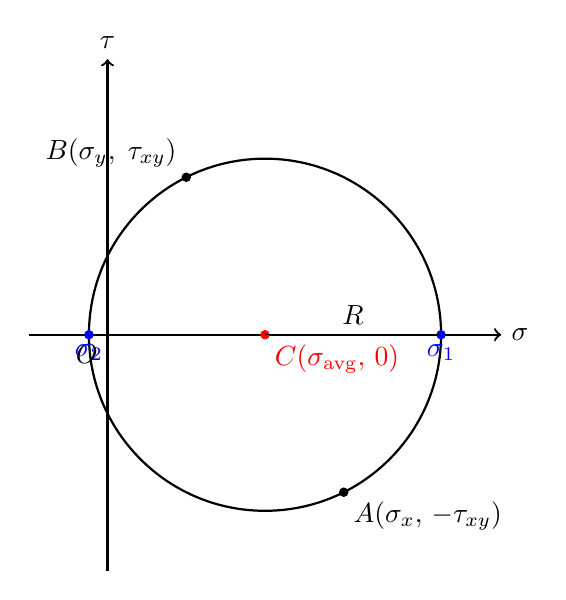
\begin{tikzpicture}[scale=1]
  % 画坐标轴
  \draw[->, thick] (-1,0) -- (5,0) node[right] {$\sigma$};
  \draw[->, thick] (0,-3) -- (0,3.5) node[above] {$\tau$};
  \node at (0,0) [below left] {$O$};

  % 示例应力状态:sigma_x = 3, sigma_y = 1, tau_xy = 2
  \def\sx{3}
  \def\sy{1}
  \def\txy{2}

  % 计算圆心和半径
  \pgfmathsetmacro\savg{(\sx+\sy)/2}
  \pgfmathsetmacro\R{sqrt(((\sx-\sy)/2)^2 + (\txy)^2)}

  % 画莫尔圆
  \draw[thick] (\savg,0) circle (\R);

  % 标记点 A 和 B
  \filldraw[black] (\sx,-\txy) circle (1.5pt) node[below right] {$A(\sigma_x,\,-\tau_{xy})$};
  \filldraw[black] (\sy,\txy) circle (1.5pt) node[above left] {$B(\sigma_y,\;\tau_{xy})$};

  % 标记圆心 C
  \filldraw[red] (\savg,0) circle (1.5pt) node[below right] {$C(\sigma_{\text{avg}},\,0)$};

  % 标记主应力点
  \filldraw[blue] ({\savg+\R},0) circle (1.5pt) node[below] {$\sigma_1$};
  \filldraw[blue] ({\savg-\R},0) circle (1.5pt) node[below] {$\sigma_2$};

  % 标注半径 R
  \draw[dashed] (\savg,0) -- ({\savg+\R},0) node[midway,above] {$R$};

\end{tikzpicture}
\caption{莫尔圆示意图:点 $A(\sigma_x,\,-\tau_{xy})$ 与 $B(\sigma_y,\;\tau_{xy})$ 均在圆上,圆心 $C$ 在 $(\sigma_{\text{avg}},\,0)$,主应力 $\sigma_{1},\,\sigma_{2}$ 分别对应最右、最左点。}
\end{figure}

\section*{9. 强度理论的分类及名称}

\subsection*{9.1 第一类强度理论(脆性断裂的理论)}

\noindent
第一强度理论——最大拉应力理论:
\[
  \sigma_{r1} \;=\; \sigma_1.
\]

\noindent
第二强度理论——最大伸长线应变理论:
\[
  \sigma_{r2} \;=\; \sigma_1 \;-\; \nu\,(\sigma_2 + \sigma_3).
\]

\subsection*{9.2 第二类强度理论(塑性屈服的理论)}

\noindent
第三强度理论——最大切应力理论:
\[
  \sigma_{r3} \;=\; \sigma_1 \;-\; \sigma_3.
\]

\noindent
第四强度理论——形状改变量能密度理论:
\[
  \sigma_{r4} \;=\; \sqrt{\frac{1}{2}\Bigl[(\sigma_1 - \sigma_2)^2 \;+\; (\sigma_2 - \sigma_3)^2 \;+\; (\sigma_3 - \sigma_1)^2\Bigr]}.
\]

\section*{10. 结构力学中的正对称与反对称}

\subsection*{10.1 定义与基本分类}

对于具有几何对称性的结构(例如梁、框架等),相对于其对称轴或对称面,可以将载荷、位移和内力分为两类:

\begin{itemize}
  \item \textbf{正对称}  
  \begin{itemize}
    \item \textbf{载荷、位移和内力沿对称轴(面)正对称分布。}  
    \item 载荷作用方向和大小在对称轴(面)两侧相同,变形形态关于对称轴(面)对称。  
    \item 内力如轴力和弯矩,沿对称轴分布且对称。  
  \end{itemize}

  \item \textbf{反对称}  
  \begin{itemize}
    \item \textbf{载荷、位移和内力关于对称轴(面)反对称分布。}  
    \item 载荷方向相反或变号,变形关于对称轴(面)呈镜像反向。  
    \item 内力如剪力、扭矩沿对称轴反对称分布。
  \end{itemize}
\end{itemize}

\subsection*{10.2 对称性对应的几何和物理特性}

\begin{table}[h]
\centering
\begin{tabular}{|c|c|c|}
\hline
\textbf{类别} & \textbf{正对称位置} & \textbf{反对称位置} \\ \hline
\textbf{荷载} & 沿对称轴 & 垂直于对称轴、弯矩 \\ \hline
\textbf{位移} & 沿对称轴 & 垂直于对称轴、转角 \\ \hline
\textbf{内力} & 轴力、垂直于对称轴的弯矩 & 剪力、沿对称轴的弯矩 \\ \hline
\end{tabular}
\caption{结构正对称与反对称载荷、位移和内力的分布特性}
\end{table}

\subsection*{10.3 内力和变形特征}

\begin{itemize}
  \item 在 \textbf{正对称载荷}作用下,结构的内力和变形均呈正对称,即载荷、位移和内力分布在对称轴(面)两侧相同。  
  \item 在 \textbf{反对称载荷}作用下,结构的内力和变形呈反对称,即载荷、位移和内力在对称轴(面)两侧大小相等但方向相反。  
  \item 由于线性力学假设,结构的总响应可由正对称和反对称两部分叠加而成,彼此互不干扰。  
\end{itemize}

\subsection*{10.4 正对称与反对称示意图(TikZ)}

\begin{figure}[h]
\centering
\begin{tikzpicture}[scale=1.2]

% 坐标轴
\draw[thick,->] (-0.5,0) -- (4.5,0) node[right] {$x$};
\draw[thick,->] (0,-2) -- (0,2) node[above] {$y$};
\node at (0,0) [below left] {$O$};

% 对称轴
\draw[dashed, thick] (2,-2) -- (2,2) node[above] {对称轴};

% 正对称载荷示意
\draw[thick,blue,->] (1,1.5) -- (1,0.5) node[left] {$F$};
\draw[thick,blue,->] (3,1.5) -- (3,0.5) node[right] {$F$};

% 正对称位移示意 (向下)
\draw[thick,red] (1,0) .. controls (1.5,-0.5) and (2.5,-0.5) .. (3,0);
\draw[thick,red] (1,0) node[left] {$u(x)$} .. controls (1.5,-0.5) and (2.5,-0.5) .. (3,0) node[right] {$u(-x)$};

% 标注
\node at (2,-1.5) {\textbf{正对称示意}};

\end{tikzpicture}
\hspace{2cm}
\begin{tikzpicture}[scale=1.2]

% 坐标轴
\draw[thick,->] (-0.5,0) -- (4.5,0) node[right] {$x$};
\draw[thick,->] (0,-2) -- (0,2) node[above] {$y$};
\node at (0,0) [below left] {$O$};

% 对称轴
\draw[dashed, thick] (2,-2) -- (2,2) node[above] {对称轴};

% 反对称载荷示意
\draw[thick,blue,->] (1,1.5) -- (1,0.5) node[left] {$F$};
\draw[thick,blue,<-] (3,-0.5) -- (3,0.5) node[right] {$-F$};

% 反对称位移示意 (一边向下,一边向上)
\draw[thick,red] (1,0) .. controls (1.5,-0.5) and (2.5,0.5) .. (3,0);
\draw[thick,red] (1,0) node[left] {$u(x)$} .. controls (1.5,-0.5) and (2.5,0.5) .. (3,0) node[right] {$-u(-x)$};

% 标注
\node at (2,-1.5) {\textbf{反对称示意}};

\end{tikzpicture}
\caption{正对称和反对称载荷与位移示意图:蓝色箭头表示载荷方向,红色曲线表示结构位移形态。}
\end{figure}

\vspace{1cm}

\begin{figure}[H]
\centering
% 内力示意图 - 正对称
\begin{tikzpicture}[scale=1]

% 梁的轴线
\draw[thick] (0,0) -- (5,0);
\draw[dashed] (2.5,-1) -- (2.5,1) node[above] {对称轴};

% 轴力和弯矩(正对称)
% 轴力
\draw[thick,blue,->] (1,0.3) -- (1,1) node[above] {$N$};
\draw[thick,blue,->] (4,0.3) -- (4,1) node[above] {$N$};

% 弯矩
\draw[thick,red] plot [smooth,tension=1] coordinates {(0,0) (1.5,0.5) (2.5,1) (3.5,0.5) (5,0)};
\node at (2.5,1.3) {$M$};

% 文字标注
\node at (2.5,-0.7) {正对称内力分布};

\end{tikzpicture}
\hspace{1.5cm}
% 内力示意图 - 反对称
\begin{tikzpicture}[scale=1]

% 梁的轴线
\draw[thick] (0,0) -- (5,0);
\draw[dashed] (2.5,-1) -- (2.5,1) node[above] {对称轴};

% 剪力和扭矩(反对称)
% 剪力
\draw[thick,blue,->] (1,0.3) -- (1,1) node[above] {$Q$};
\draw[thick,blue,<-] (4,0.3) -- (4,1) node[above] {$-Q$};

% 扭矩
\draw[thick,red] plot [smooth,tension=1] coordinates {(0,0) (1.5,0.5) (2.5,1) (3.5,0.5) (5,0)};
\node at (2.5,1.3) {$T$};

% 文字标注
\node at (2.5,-0.7) {反对称内力分布};

\end{tikzpicture}
\caption{结构内力的正对称与反对称分布示意图。蓝色箭头代表轴力、剪力,红色曲线代表弯矩、扭矩分布。}
\end{figure}


% 以下按前述格式,输出组合变形的公式,包括轴向、弯曲和扭转等变形的叠加关系和示例。

% 文档结束

\section*{11. 问答题回答及知识点介绍}

\subsection*{第一章 绪论及基本概念}
\begin{itemize}
  \item \textbf{可变形固体的基本假设}:假设固体材料连续、均匀且各点位移连续,变形过程中体积变化很小,忽略材料内部微观结构对宏观力学行为的影响。
  \item \textbf{杆件变形的基本形式}:包括轴向变形(拉伸、压缩)、弯曲变形、扭转变形以及剪切变形。
\end{itemize}

\subsection*{第二章 轴向拉伸和压缩}
\begin{itemize}
  \item \textbf{正应力、切应力、平均应力的定义}:
    \begin{itemize}
      \item 正应力:垂直于截面的内力单位面积上的分布;
      \item 切应力:平行于截面的内力单位面积上的分布;
      \item 平均应力:内力除以截面面积的值,代表平均分布应力。
    \end{itemize}
  \item \textbf{圣维南原理}:在杆件的某一截面处,截面以外的力及力矩对该截面的应力分布无影响。
  \item \textbf{胡克定律及其物理意义}:
    \begin{itemize}
      \item 关系式:应力与应变成正比,线性弹性阶段有效;
      \item 单轴应力状态下,$\sigma = E \varepsilon$,其中$E$为弹性模量。
    \end{itemize}
  \item \textbf{低碳钢拉伸试验的应力应变曲线及四阶段}:
    \begin{itemize}
      \item 四阶段:弹性阶段、屈服阶段、强化阶段、断裂阶段;
      \item 比例极限:应力应变曲线开始偏离直线的点;
      \item 弹性极限:最大弹性应力;
      \item 上屈服强度:屈服曲线上升峰值;
      \item 下屈服强度:屈服期间,不计初始瞬时效应的最小应力;
      \item 屈服极限:材料开始发生塑性变形的应力;
      \item 强度极限:材料能承受的最大应力;
      \item 断后伸长率:断裂前伸长的长度与原始长度比;
      \item 断面收缩率:断裂时横截面缩小面积与原始面积比。
    \end{itemize}
  \item \textbf{应力集中的概念}:由于几何突变、缺口等造成的局部应力增大现象。
\end{itemize}

\subsection*{第三章 扭转}
\begin{itemize}
  \item \textbf{扭转截面系数}:描述截面抗扭能力的参数。
  \item \textbf{切应力互等定理}:在纯扭转条件下,截面各点切应力大小相等。
  \item \textbf{翘曲的定义}:非圆截面扭转时截面出现的非平面变形。
  \item \textbf{形心、静矩、惯性矩、惯性半径、惯性积、主惯性矩、形心主惯性矩的定义}:
    \begin{itemize}
  \item \textbf{形心}:截面面积的几何中心,即截面上所有微小面积元素的位置矢量的面积加权平均点。形心的位置使得截面对该点的静矩为零。
  \item \textbf{静矩}(第一面积矩):截面上某一部分面积相对于某轴的第一矩,计算公式为
  \[
    Q = \int y \, dA
  \]
  其中$y$是该面积元相对于参考轴的垂直距离。静矩用于计算截面受力时的弯矩作用。
  \item \textbf{惯性矩}(第二面积矩):截面面积对某轴的第二矩,定义为
  \[
    I = \int y^2 \, dA
  \]
  表征截面抵抗弯曲变形的能力,数值越大,截面抗弯刚度越强。
  \item \textbf{惯性半径}:截面对某轴的惯性矩$I$与截面面积$A$的比值的平方根,表示截面面积相对于该轴的分布特征,计算公式为
  \[
    r = \sqrt{\frac{I}{A}}.
  \]
  惯性半径反映截面面积“离开”该轴的平均距离。
  \item \textbf{惯性积}(积矩):截面对两个不同轴(如$x$轴和$y$轴)的混合二阶面积矩,定义为
  \[
    I_{xy} = \int xy \, dA,
  \]
  它描述截面相对于两个坐标轴的耦合性质,当惯性积不为零时,轴向的弯曲相互影响。
  \item \textbf{主惯性矩}:通过旋转坐标轴,找到一组坐标轴使惯性积为零时,这组坐标轴对应的惯性矩称为主惯性矩。主惯性矩代表截面在这组主轴方向上的最大和最小抗弯刚度。
  \item \textbf{形心主惯性矩}:是在形心坐标系下的主惯性矩,即通过形心且使惯性积为零的主轴上的惯性矩,常用于结构分析和设计中。
\end{itemize}
\end{itemize}

\subsection*{第四章 弯曲应力}
\begin{itemize}
  \item \textbf{对称弯曲与非对称弯曲}:对称弯曲是弯矩与截面主惯性轴对应,非对称弯曲则不对应。
  \item \textbf{叠加原理}:线性系统中,总变形或应力等于各载荷单独作用的叠加。
  \item \textbf{纯弯曲与横力弯曲的区别}:纯弯曲无剪力,横力弯曲存在剪力。
  \item \textbf{纯弯曲时平面假设,中性轴及中性层定义}:
    \begin{itemize}
      \item 平面假设:截面变形仍保持平面;
      \item 中性轴:弯曲截面中无应力的轴线;
      \item 中性层:截面内应变为零的层面。
    \end{itemize}
  \item \textbf{梁截面上切应力两个假设}:
    \begin{itemize}
      \item 剪应力分布较均匀;
      \item 剪应力主要作用于中性层。
    \end{itemize}
  \item \textbf{梁合理设计的工程措施}:截面合理选择,材料合理利用,加强局部支撑,减小应力集中等。
\end{itemize}

\subsection*{第五章 梁弯曲时的位移}
\begin{itemize}
  \item \textbf{提高梁刚度的措施}:增加截面惯性矩,选用高模量材料,合理支撑及加劲等。
\end{itemize}

\subsection*{第六章 简单的超静定问题}
\begin{itemize}
  \item \textbf{静定问题、超静定问题及相关定义}:
    \begin{itemize}
      \item 静定问题:支持反力数等于平衡方程数;
      \item 超静定问题:支持反力数超过平衡方程数,多余约束;
      \item “多余”约束:超出平衡要求的约束;
      \item 超静定次数:多余约束数;
      \item 基本静定系:移除多余约束后的结构。
    \end{itemize}
  \item \textbf{装配内力与装配应力}:因结构装配引起的内力和应力。
  \item \textbf{温度内力与温度应力}:温度变化引起的内力和应力。
\end{itemize}

\subsection*{第七章 应力状态与强度理论}
\begin{itemize}
  \item \textbf{应力状态定义}:材料内部应力的分布形态,平面应力状态是二维应力状态,空间应力状态是三维应力状态。
  \item \textbf{应力圆方程及图示(莫尔圆)}:
  \[
    (\sigma_x - \sigma_{\text{avg}})^2 + \tau_{xy}^2 = R^2,
  \]
  其中,$\sigma_{\text{avg}} = \frac{\sigma_x + \sigma_y}{2}$,半径$R = \sqrt{\left(\frac{\sigma_x - \sigma_y}{2}\right)^2 + \tau_{xy}^2}$。
  \item \textbf{主平面及主应力}:使切应力为零的平面上的正应力即为主应力。
  \item \textbf{四个常用强度理论及等效应力表达式}:
    \begin{itemize}
      \item 最大正应力理论;
      \item 最大剪应力理论;
      \item 最大主应变能密度理论;
      \item 最大扭转能理论(冯·米塞斯准则)。
    \end{itemize}
\end{itemize}

\subsection*{第八章 组合变形及连接部分的计算}
\begin{itemize}
  \item \textbf{组合变形与连接件定义}:多种变形方式同时存在,连接件为构件间连接部分。
  \item \textbf{偏心拉伸或压缩}:载荷作用线不通过截面形心导致弯矩。
  \item \textbf{截面核心定义}:截面内使偏心载荷仍产生纯压力不发生拉应力的区域。
  \item \textbf{螺栓连接三种破坏形式}:螺栓剪切破坏、螺栓拉断、连接板剪切破坏。
  \item \textbf{铆钉连接三种方式}:单铆钉连接、双铆钉连接及多排铆钉连接。
\end{itemize}

\subsection*{第九章 压杆稳定}
\begin{itemize}
  \item \textbf{平衡三种状态}:稳定平衡、临界平衡、不稳定平衡。
  \item \textbf{临界平衡及临界力}:临界状态是系统处于边界平衡状态,临界力为使杆失稳的最小载荷。
  \item \textbf{欧拉公式及适用范围}:
  \[
  P_{\text{cr}} = \frac{\pi^2 EI}{(KL)^2},
  \]
  其中$E$为弹性模量,$I$惯性矩,$L$有效长度,$K$长度系数。适用于长细比大的压杆。
  \item \textbf{提高压杆稳定性措施}:增加截面惯性矩,缩短有效长度,增加支撑等。
\end{itemize}

\subsection*{第一章 弯曲问题的进一步研究}
\begin{itemize}
  \item \textbf{平面弯曲与斜弯曲}:平面弯曲弯矩作用在主惯性轴上,斜弯曲则不在主惯性轴上。
  \item \textbf{相当截面定义}:折算成等效截面以简化复杂截面分析。
  \item \textbf{弯曲中心定义}:作用力使梁弯曲而不产生扭转的点。
\end{itemize}

\subsection*{第二章 考虑材料塑性的极限分析}
\begin{itemize}
  \item \textbf{永久变形及残余应力}:超过弹性极限的塑性变形,卸载后仍保留的应力。
  \item \textbf{简单加载及极限状态}:逐步加大载荷,直至结构失稳或破坏的状态。
  \item \textbf{弹性-理想塑性模型与刚性-理想塑性模型}:前者有弹性阶段,后者无弹性阶段直接塑性变形。
  \item \textbf{屈服荷载与极限荷载}:屈服荷载为材料开始屈服时载荷,极限荷载为极限承载能力。
  \item \textbf{屈服扭矩与极限扭矩}:对应于材料开始屈服和极限承载能力的扭矩。
  \item \textbf{屈服弯矩与极限弯矩}:对应于材料开始屈服和极限承载能力的弯矩。
  \item \textbf{塑性弯曲截面系数}:反映截面塑性承载能力的系数。
  \item \textbf{塑性铰定义}:构件发生塑性转动的铰接区域。
\end{itemize}

\subsection*{第三章 能量法}
\begin{itemize}
  \item \textbf{几何非线性弹性问题与物理非线性弹性问题}:前者考虑大变形几何效应,后者考虑材料非线性。
  \item \textbf{卡氏第一定理、第二定理、余能定理及适用范围}:
    \begin{itemize}
      \item 第一、二定理为虚功原理的不同表达;
      \item 余能定理用于计算结构的变形能。
    \end{itemize}
  \item \textbf{力法与位移法定义}:
    \begin{itemize}
      \item 力法:选定多余力作为未知量;
      \item 位移法:选定位移或转角作为未知量。
    \end{itemize}
\end{itemize}

\subsection*{第六章 动荷载·交变应力}
\begin{itemize}
  \item \textbf{动荷载,交变应力,疲劳破坏及疲劳寿命定义}:
    \begin{itemize}
      \item 动荷载:随时间变化的载荷;
      \item 交变应力:正负交替变化的应力;
      \item 疲劳破坏:材料因循环应力导致的破坏;
      \item 疲劳寿命:材料在交变应力下能承受的循环次数。
    \end{itemize}
  \item \textbf{冲击作用定义}:短时间内产生的大幅度载荷作用。
  \item \textbf{应力谱,应力循环,应力比,应力幅定义}:
    \begin{itemize}
      \item 应力谱:某段时间内应力的变化范围;
      \item 应力循环:一次完整的应力变化过程;
      \item 应力比:最小应力与最大应力之比;
      \item 应力幅:应力最大值与最小值差的一半。
    \end{itemize}
\end{itemize}

\subsection*{第七章 材料力学性能的进一步研究}
\begin{itemize}
  \item \textbf{蠕变与松弛定义}:
    \begin{itemize}
      \item 蠕变:恒定载荷下材料随时间缓慢变形;
      \item 松弛:恒定应变下材料应力随时间减小。
    \end{itemize}
\end{itemize}


\newpage

%=================== 题目部分 ===================
\begin{questions}
    \item 两铸件用两钢杆1、2连接,其间距\( l = 200mm \)(图a)。现需将制造得过长(\(\Delta e = 0.11mm\))的铜杆3(图b)装入铸件之间,并保持三杆的轴线平行且有等间距\( a \)。已知:钢杆直径\( d = 10mm \),铜杆横截面为\( 20mm \times 30mm \)的矩形,钢的弹性模量\( E = 210GPa \),铜的弹性模量\( E_3 = 100GPa \)。铸件很厚,其变形可略去不计。试计算各杆内的装配应力。\\(\textbf{拉压超静定问题})
    
    \begin{figure}[H]
        \centering
        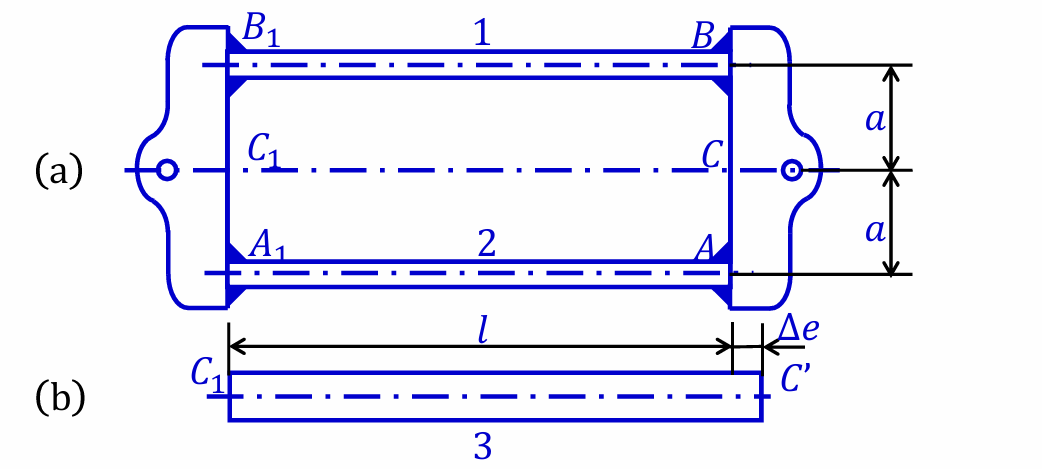
\includegraphics[width=0.7\textwidth]{figures/1.png}
    \end{figure}

    \item 两端直径分别为\( d_1 = 40mm \)和\( d_2 = 80mm \),长度\( l = 1m \)的锥形圆杆,与外直径\( D = 120mm \),中心具有相同锥形圆孔的空心圆杆配合成组合杆,如图所示。组合杆在两端承受扭转外力偶矩\( M_e = 5kN \cdot m \)作用。设两杆在接触面为紧密配合,不发生相对转动,且两杆的切变模量之比为\( G_1 / G_2 = 1/2 \),试求实心锥形圆杆内的最大切应力。\\(\textbf{拉压超静定问题,带温度效应})

    \begin{figure}[H]
        \centering
        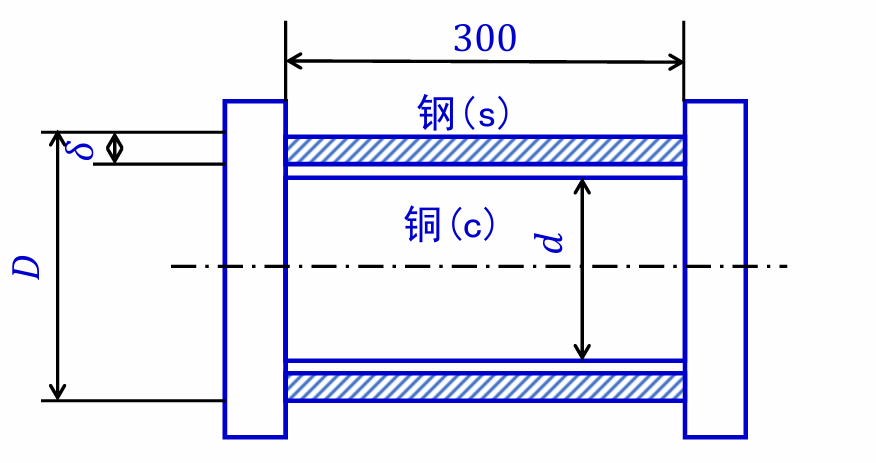
\includegraphics[width=0.7\textwidth]{figures/2.png}
    \end{figure}

    \item 两端直径分别为\( d_1 = 40mm \)和\( d_2 = 80mm \), 长度\( l = 1m \)的锥形圆杆, 与外直径\( D = 120mm \), 中心具有相同锥形圆孔的空心圆杆配合成组合杆, 如图所示。组合杆在两端承受扭转外力偶矩\( M_e = 5kN \cdot m \)作用。设两杆在接触面为紧密配合, 不发生相对转动, 且两杆的切变模量之比为\( G_1 / G_2 = 1/2 \), 试求实心锥形圆杆内的最大切应力。\\(\textbf{扭转超静定问题,配合切面转角相同})
    
    \begin{figure}[H]
        \centering
        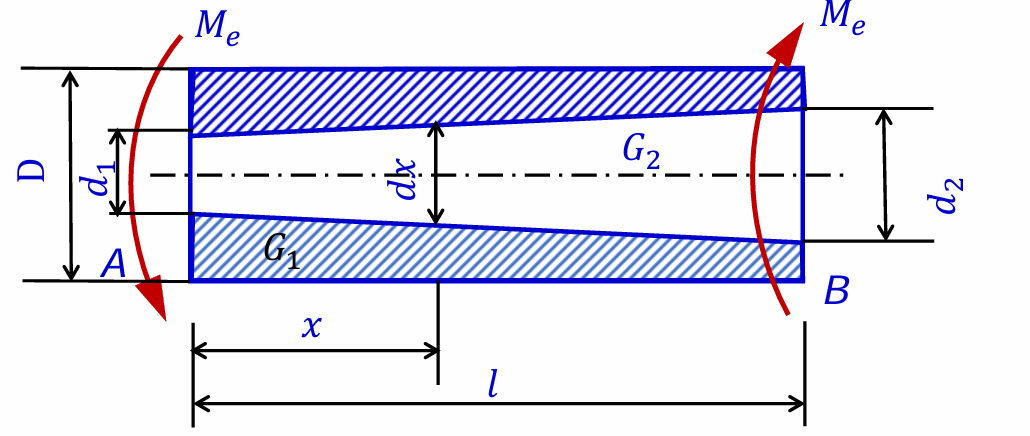
\includegraphics[width=0.7\textwidth]{figures/3.png}
    \end{figure}

    \item 两端简支的焊接工字钢梁及其荷载如图所示,梁的横截面尺寸示于图c中。试用应力圆求梁危险截面上a和b两点处的主应力,并绘出主应力单元体。\\  (\textbf{应力状态,莫尔圆})
    
    \begin{figure}[H]
        \centering
        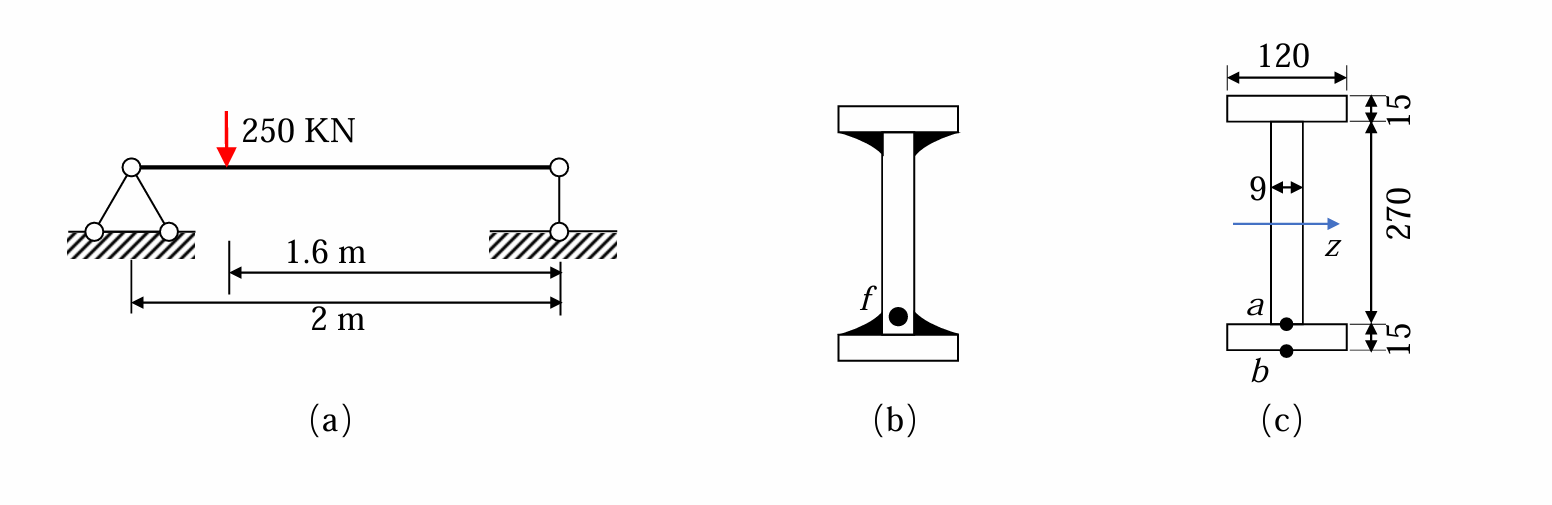
\includegraphics[width=0.7\textwidth]{figures/4.png}
    \end{figure}

    \item 一两端密封的圆柱形压力容器,圆筒部分由壁厚为δ,宽度为b的塑条滚压成螺旋状并熔接而成。圆筒的内直径为$D$,且$\delta \ll D$。容器承受的内压的压强为$p$,若熔接部分承受的拉应力不得超过塑条中最大拉应力的80\%,试求塑条的许可宽度b。\\  (\textbf{应力状态,莫尔圆})

    \begin{figure}[H]
        \centering
        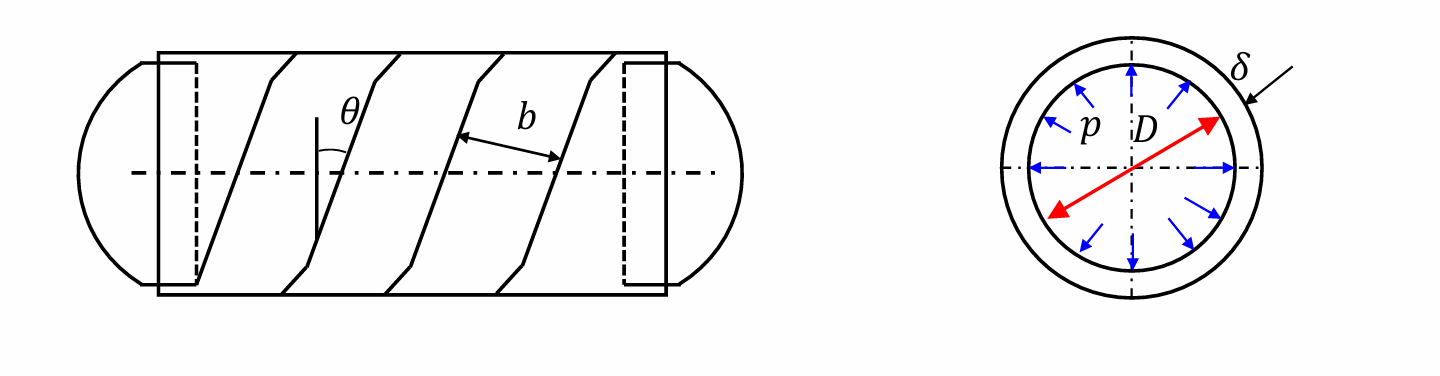
\includegraphics[width=0.7\textwidth]{figures/5.png}
    \end{figure}

    \item 两端简支的工字钢梁承受荷载如图所示。已知材料 Q235 钢的许用应力[σ]=170 MPa 和[τ]=100MPa。试按强度条件选择工字钢的型号。\\  (\textbf{强度理论,强度条件})
    
    \begin{figure}[H]
        \centering
        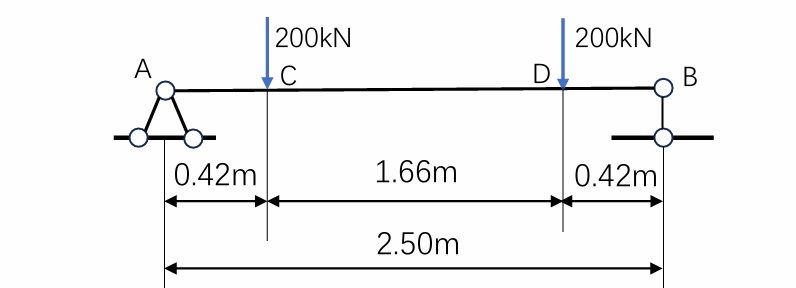
\includegraphics[width=0.7\textwidth]{figures/6.png}
    \end{figure}
    
    \item 材料为线弹性,弯曲刚度为 \(EI\) 的各超静定刚架分别如图所示,不计轴力和剪力的影响,试用卡氏第二定理求刚架的支反力。\\  (\textbf{超静定刚架,卡氏第二定理,注意变形关系,所以左右的水平力是相同的,第二个涉及对称性,看我前面笔记})
    
    \begin{figure}[H]
        \centering
        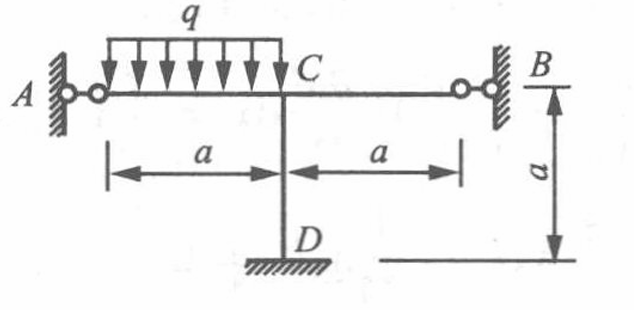
\includegraphics[width=0.7\textwidth]{figures/7.png}
    \end{figure}
    \begin{figure}[H]
        \centering
        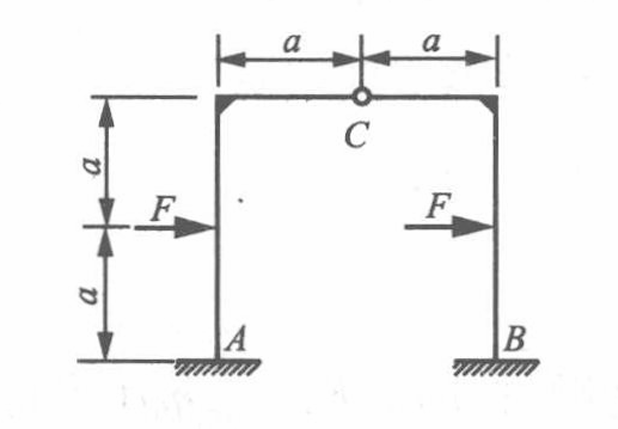
\includegraphics[width=0.7\textwidth]{figures/8.png}
    \end{figure}

    \item 刚度为EI的悬臂梁,见下图,已知其自由端的转角为$\theta$。梁材料为线弹性,利用卡氏第一定理确定外力偶矩$Me$。\\ (\textbf{形变的几何关系,卡式第一定理})
    
    \begin{figure}[H]
        \centering
        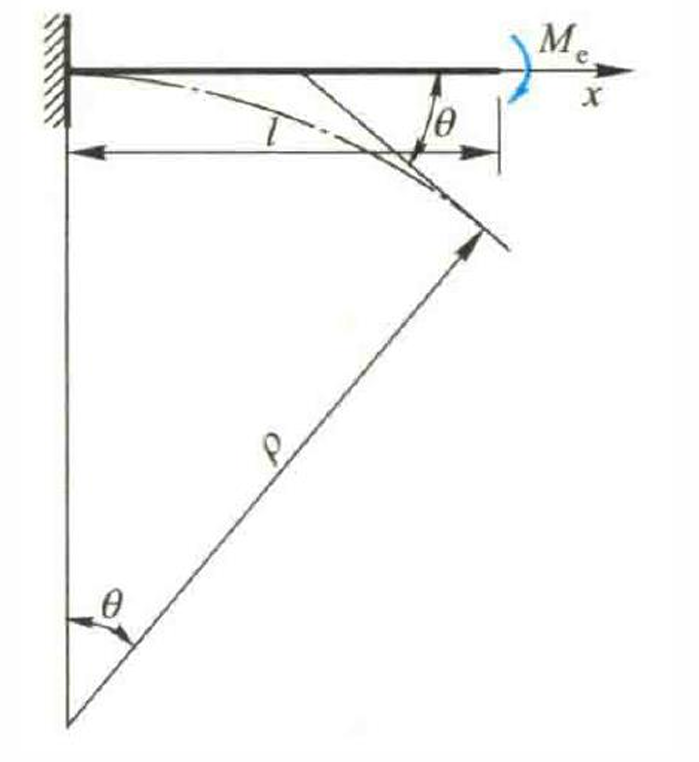
\includegraphics[width=0.4\textwidth]{figures/9.png}
    \end{figure}

    \item 图 8-42a 所示三杆支架,下部悬挂一重量为 W 的重物。已知三杆材料相同,1 杆和 2 杆的截面积均为 A。试确定 3 杆的截面积,以使重物只发生竖向位移而无水平位移,并计算此时三杆的内力。 \\ (\textbf{超静定结构,结构力学,直接上几何条件})
    
    \begin{figure}[H]
        \centering
        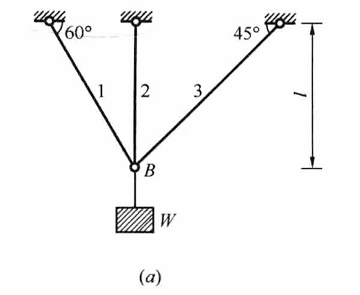
\includegraphics[width=0.4\textwidth]{figures/10.png}
    \end{figure}

    \item 圆弧形曲杆受力如图所示。已知曲杆的轴线为圆弧,其半径为 R,试写出任意横截面 C 上剪力、弯矩和轴力的表达式(表示成 $\phi$角的函数),并作曲杆的剪力图、弯矩图和轴力图。 \\ (\textbf{曲杆受力分析,剪力图,弯矩图,轴力图、弯矩的方向判断})
    
    \begin{figure}[H]
        \centering
        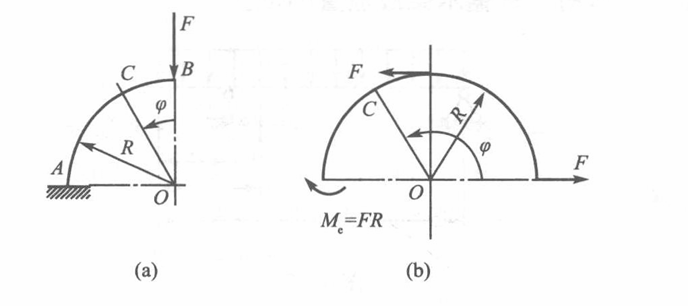
\includegraphics[width=0.4\textwidth]{figures/11.png}
    \end{figure}

    \item 如图所示圆锥形杆受轴向拉力作用,试求杆的伸长。 \\ (\textbf{轴向拉力,伸长计算})
    
    \begin{figure}[H]
        \centering
        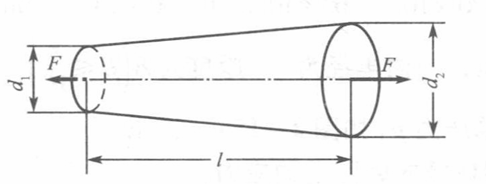
\includegraphics[width=0.6\textwidth]{figures/12.png}
    \end{figure}
    
    \item 如图所示,一内半径为 r,厚度为 δ(δ≤r/10),宽度为 b 的薄壁圆环。在圆环的内表面承受均匀分布的压力 p(如图 2-15),试求:
    \begin{itemize}
      \item 由内压力引起的圆环径向截面上的应力
      \item 由内压力引起的圆环半径的增大
    \end{itemize}

    \begin{figure}[H]
        \centering
        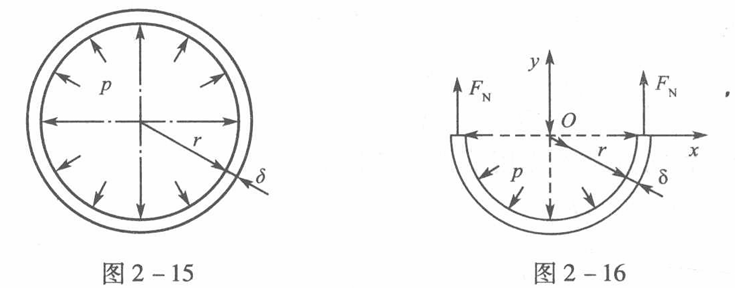
\includegraphics[width=0.6\textwidth]{figures/13.png}
    \end{figure}
    
    \item 横截面面积$A$,壁厚$\delta$,长度l和材料的切变模量均相同的三种截面形状的闭口薄壁杆,如下图所示。若分别在杆的两端承受相同的扭转外力偶矩 \( M_e \) 作用,试求三杆横截面上的切应力之比和单位长度扭转角之比。 \\ (\textbf{薄壁杆扭转,切应力,单位长度扭转角})
    
    \begin{figure}[H]
        \centering
        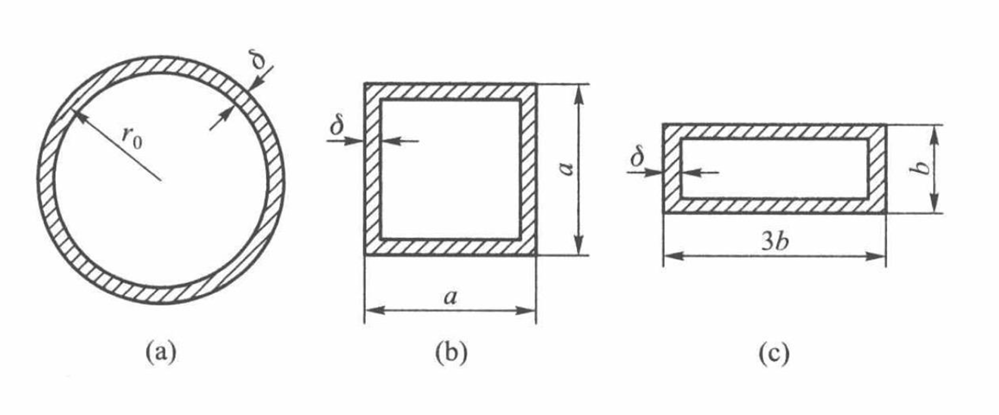
\includegraphics[width=0.6\textwidth]{figures/14.png}
    \end{figure}

    \item \begin{itemize}
      \item 试证明受轴向拉伸(压缩)的圆截面杆横截面沿圆周方向的线应变 \(\varepsilon_s\) 等于直径方向的线应变 \(\varepsilon_d\)。

      \item 一根直径为 \(d = 10\, \text{mm}\) 的圆截面杆,在轴向拉力 \(F\) 作用下,直径减小 \(0.0025\, \text{mm}\)。如材料的弹性模量 \(E = 210\, \text{GPa}\),泊松比 \(\nu = 0.3\)。试求轴向拉力 \(F\)。

      \item 空心圆截面钢杆,外直径 \(D = 120\, \text{mm}\),内直径 \(d = 60\, \text{mm}\),材料的泊松比 \(\nu = 0.3\)。当其受轴向拉伸时,已知纵向线应变 \(\varepsilon = 0.001\),试求其变形后的壁厚 \(\delta\)。
    \end{itemize}

    \item 图2-18所示结构中,AB为水平放置的刚性杆,杆1,2,3材料相同,其弹性模量E=210GPa,已知l=1m,A1=A2=100mm2,A3=150mm2,F=20kN。试求C点的水平位移和铅垂位移。 \\ (\textbf{超静定结构,水平位移,铅垂位移})
    
    \begin{figure}[H]
        \centering
        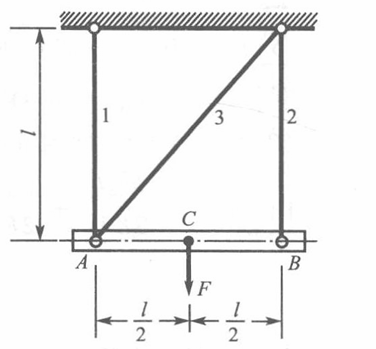
\includegraphics[width=0.6\textwidth]{figures/15.png}
    \end{figure}

    \item 图2-20所示实心圆钢杆AB和AC在A点以铰相连接,在A点作用有铅垂向下的力F=35kN。已知杆AB和AC的直径分别为d1=12mm和d2=15mm,钢的弹性模量E=210Gpa。试求A点在铅垂方向的位移。 \\ (\textbf{超静定结构,铰接连接,铅垂位移})
    
    \begin{figure}[H]
        \centering
        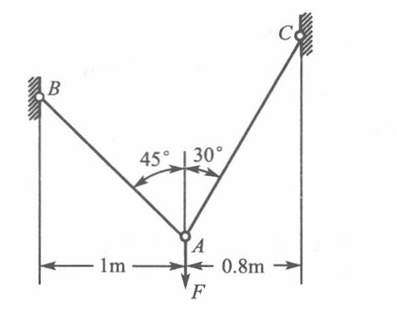
\includegraphics[width=0.6\textwidth]{figures/16.png}
    \end{figure}

    \item 如图所示,为薄壁杆的两种不同形状的横截面,其壁厚及管壁中线的周长均相同,两杆的长度和材料也相同,当在两端承受相同的一对扭转外力偶矩时,试求:
    \begin{itemize}
      \item 最大切应力之比
      \item 相对扭转角之比
    \end{itemize}

    \begin{figure}[H]
        \centering
        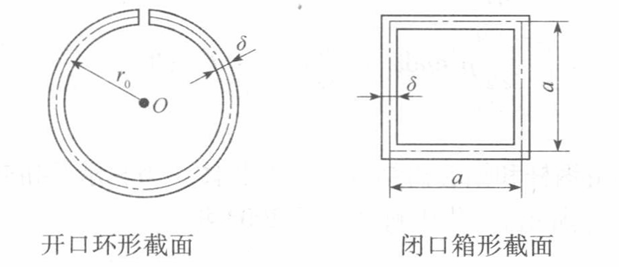
\includegraphics[width=0.6\textwidth]{figures/17.png}
    \end{figure}
\end{questions}



\newpage

%=================== 答案部分 ===================


\end{document}
%================= 结束 =================%
